% Copyright 2019 Clara Eleonore Pavillet

% Author: Clara Eleonore Pavillet
% Description: This is an unofficial Oxford University Beamer Template I made from scratch. Feel free to use it, modify it, share it.
% Version: 1.0

\documentclass{beamer}
\usepackage{verbatim}
\newenvironment{metaverbatim}{\verbatim}{\endverbatim}
% Load Packages
\usepackage[utf8]{inputenc}
\usepackage{xcolor}
\usepackage{tikz}
\usetikzlibrary{positioning,calc}
\usepackage{graphicx}
\usepackage{hyperref}
\usepackage{amsmath}
\usepackage{listings}
\usepackage{fontawesome}

% Define Commands
\newcommand*{\ClipSep}{0.06cm} %To adjust footer logo
\newcommand{\E}{\mathrm{e}\,} %\def\I{e} % used to defined e for exp(x), see later what it should be
\newcommand{\ud}{\mathrm{d}}
\lstset{numbers=left, numberstyle=\tiny, stepnumber=1,firstnumber=1,breaklines=true,
    numbersep=5pt,language=Python,
    stringstyle=\ttfamily,
    basicstyle=\footnotesize, 
    showstringspaces=false
}

\usetheme{Madrid}

\title{Dolo for absolutely beginners}
% \titlegraphic{
\includegraphics[width=2cm]{Theme/Logos/OxfordLogoV1.png}}
\author{Euiyoung Jung}
\institute{PSE}
\date{} %\today

\begin{document}

{\setbeamertemplate{footline}{} 
\frame{\titlepage}}

% \section*{Outline}\begin{frame}{Outline}\tableofcontents\end{frame}

\begin{frame}{Introduction}
    \begin{itemize}
        \item If you do not have any prior knowledge about \textit{Dolo} and try to follow the instruction provided by the program developer, you will almost always encounter error messages from the very beginning. 
        \item For example, you can find the following instruction in order to verify whether installation is done well or not. 
        \item Unfortunately, it will not work! It is because the default \textit{YAML} page in the manual is expired.
    \end{itemize}
    \end{frame}
\begin{frame}
     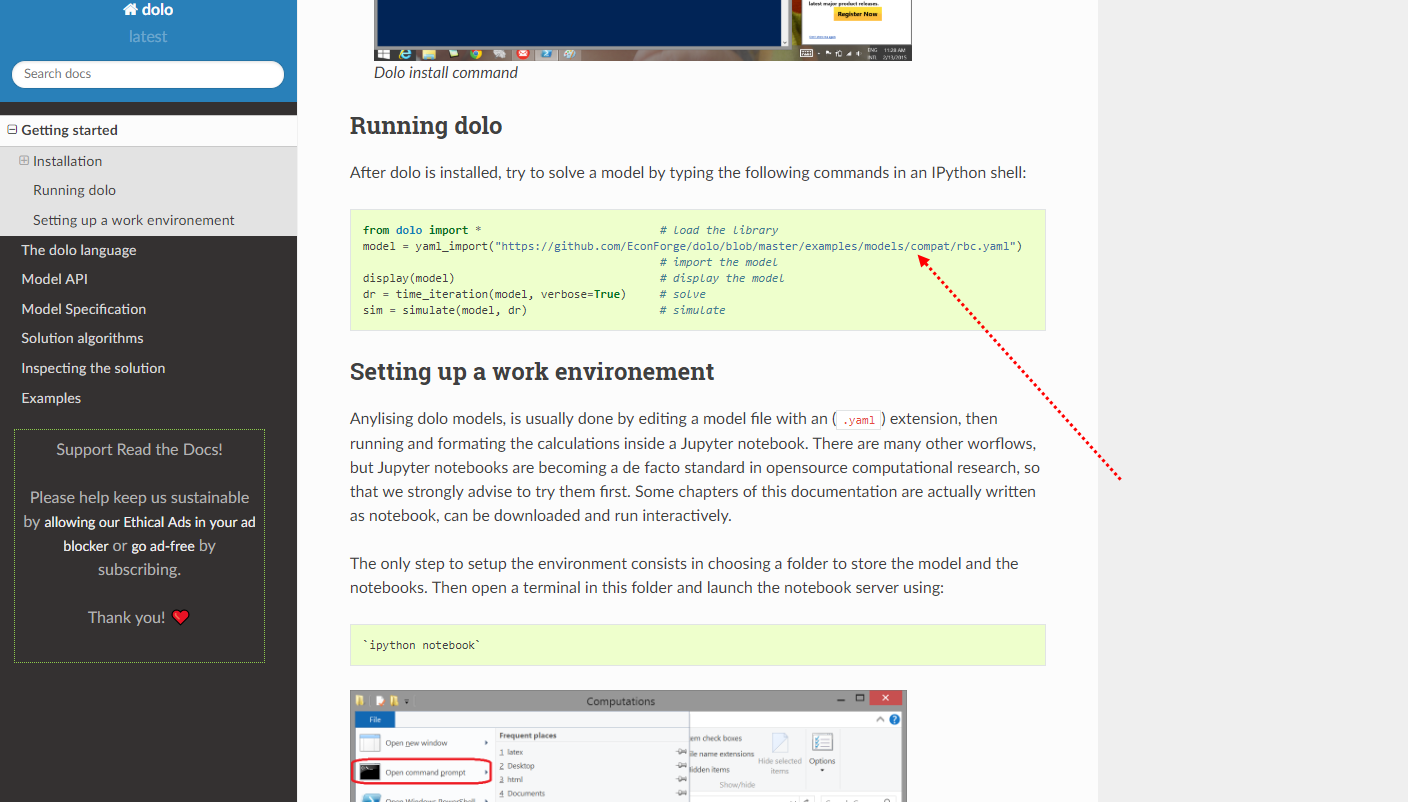
\includegraphics[width=12cm, height= 8cm]{dolo4.png} 
\end{frame}
\begin{frame}
    \begin{itemize}
    \item Instead of the \textit{YAML} address in the manual, use this url: \url{https://github.com/EconForge/dolo/blob/master/examples/models/rbc.yaml}  
    \item Your installation might be done well if \textit{Dolo} is running without error messages, once you try with url given above. 
        \item In order to write down your own model, the first step you have to do is making a github repository.
        \item Note: You have to make your repository \textbf{public}. Otherwise, your local python like \textit{Jupyter notebook} cannot call your \textit{YAML} file. 
        \item Let's start from basic housechores step by step. 
    \end{itemize}
\end{frame}
  \begin{frame}{Making a Github repository}
           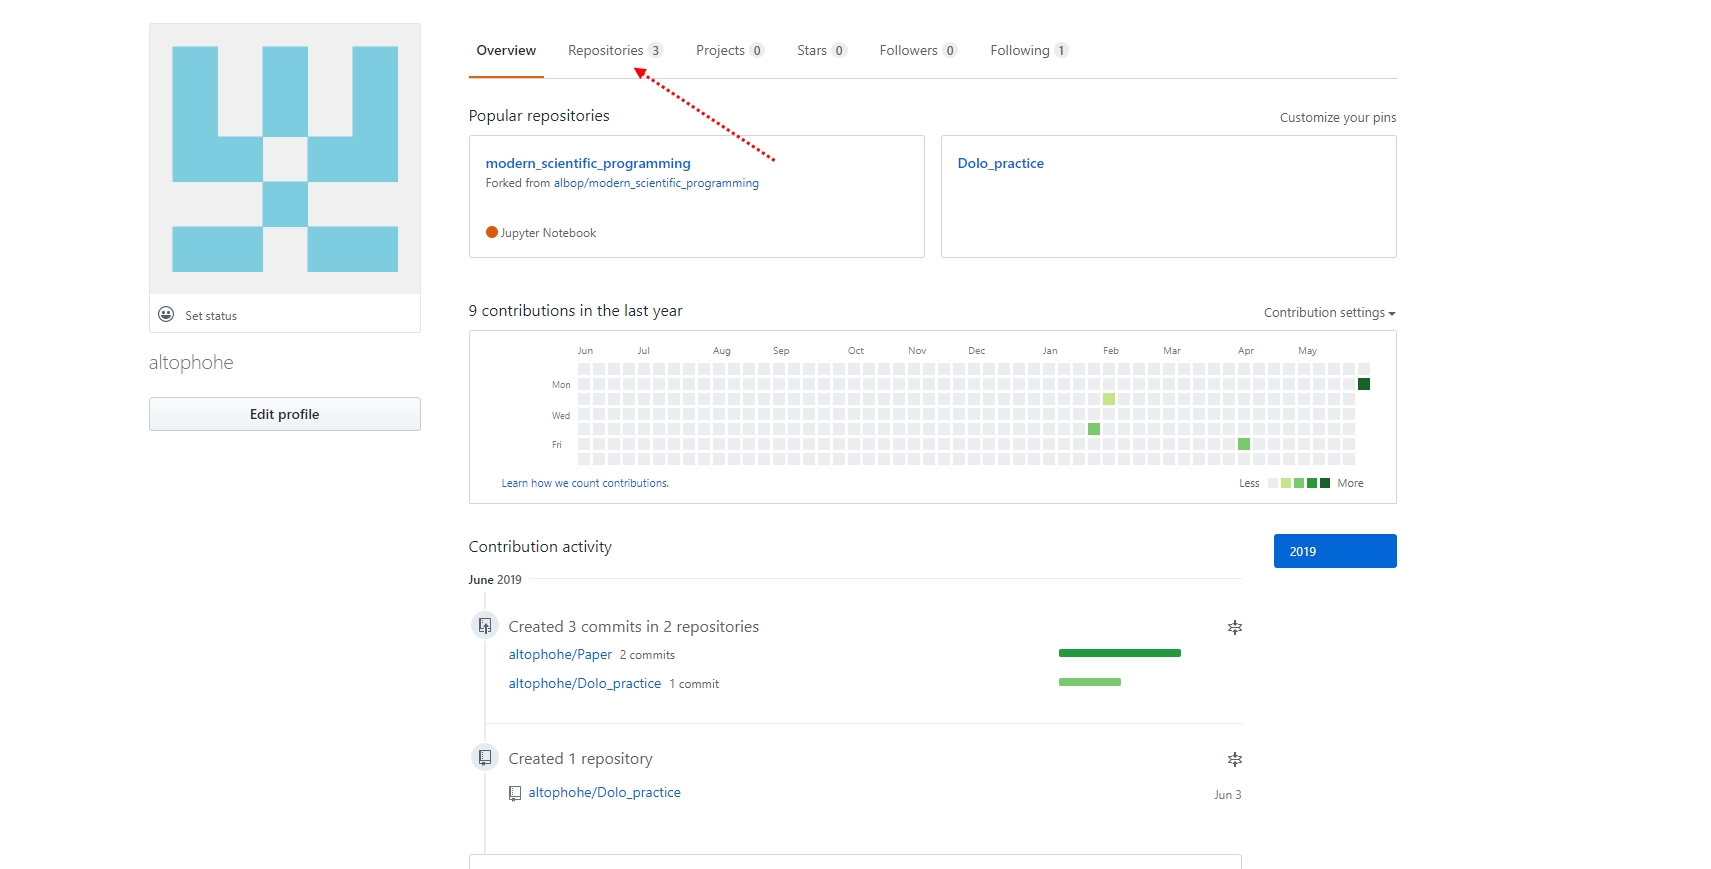
\includegraphics[width=12cm, height= 8cm]{dolo1.jpg} 
    \end{frame}
    \begin{frame}{Making a Github repository}
           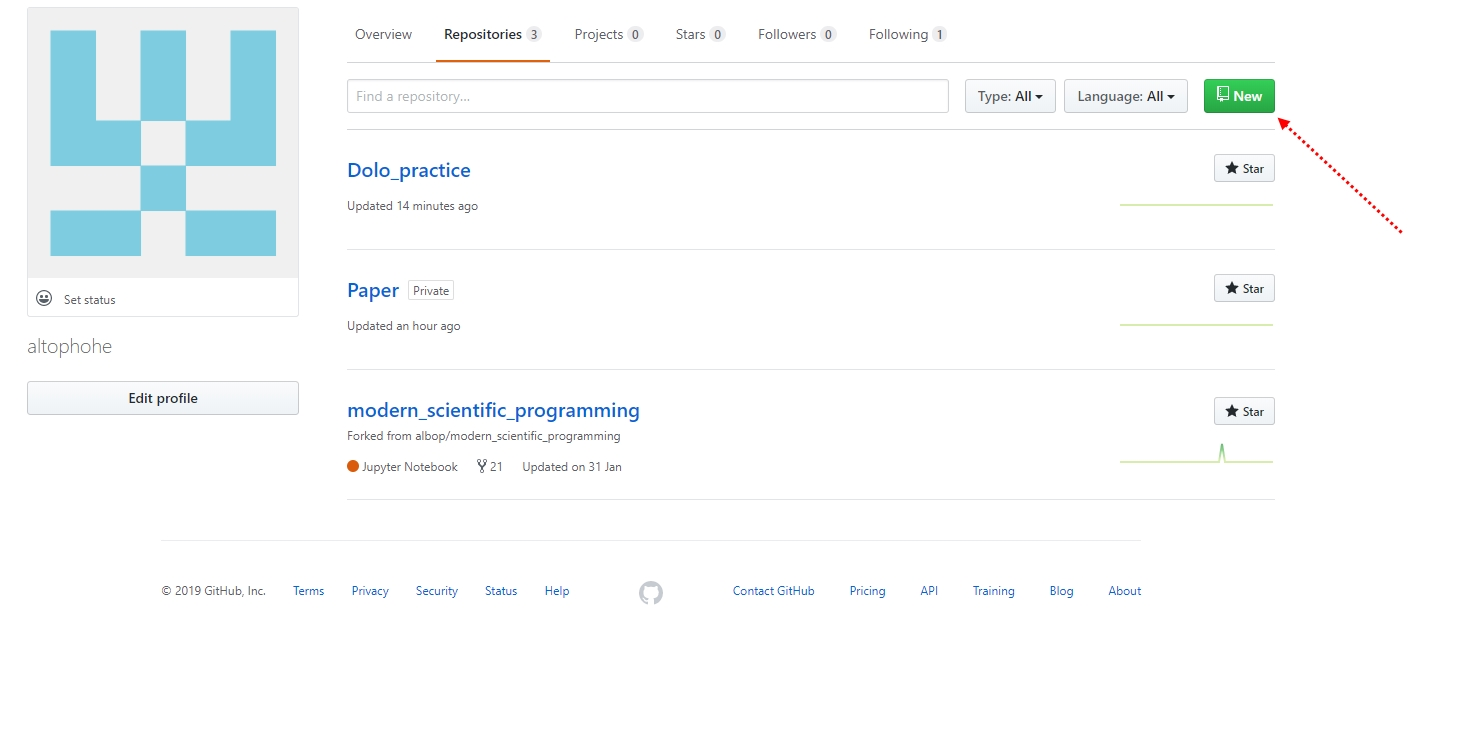
\includegraphics[width=12cm, height= 8cm]{dolo2.jpg} 
    \end{frame}
     \begin{frame}{Making a Github repository}
           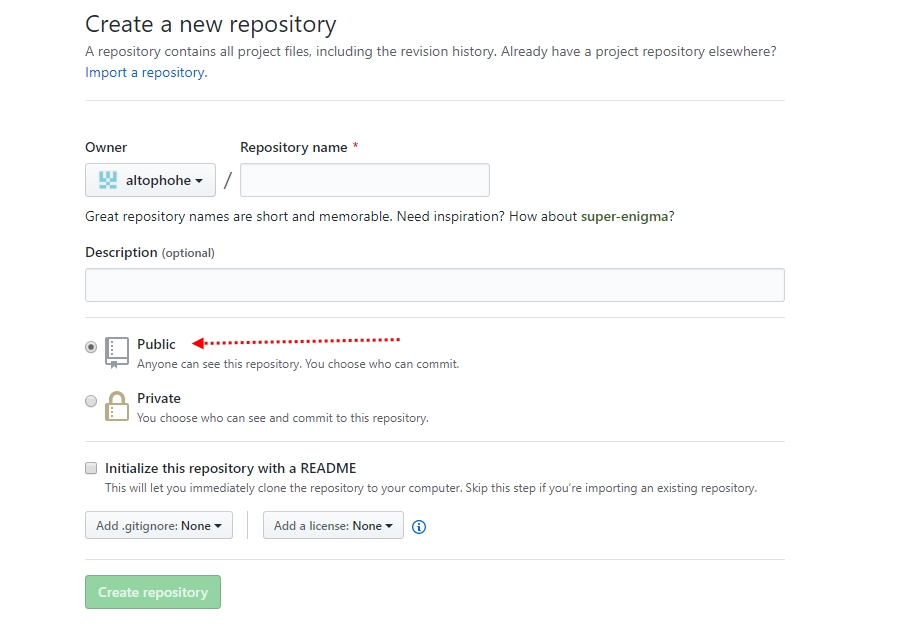
\includegraphics[width=12cm, height= 8cm]{dolo3.jpg} 
    \end{frame}
  
\begin{frame}{Making a Github repository}
    \begin{itemize}
    \item If you could manage to do all steps so far, now you made your own Github repository. 
    \item You can write your own \textit{YAML} file which would be the the backbone of Dolo computation.
        \item The easiest way to start is utilizing examples provided by the developer. You can find several examples from Pablo Winant's Github repository. 
        \item The Dolo language and the way to write down the model can be found at \url{https://dolo.readthedocs.io/en/latest/}
        \item Writing an \textit{YAML} model file in your own repository may not be easy. Let's start from Pablo Winant's examples. 
    \end{itemize}
\end{frame}
    \begin{frame}{Dolo examples}
 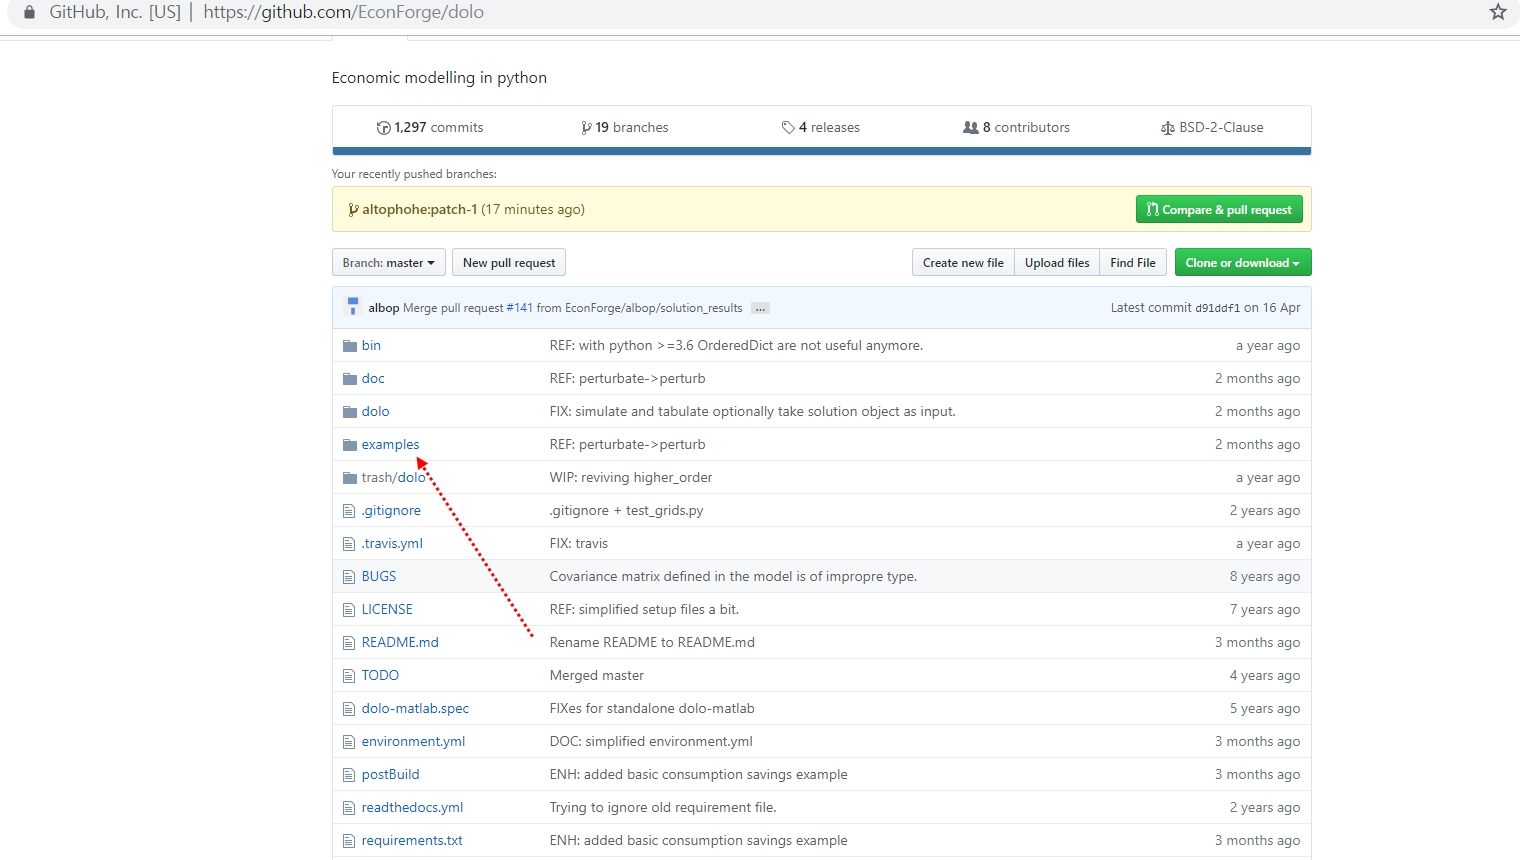
\includegraphics[width=12cm, height= 8cm]{dolo5.jpg}
    \end{frame}
    \begin{frame}{}
         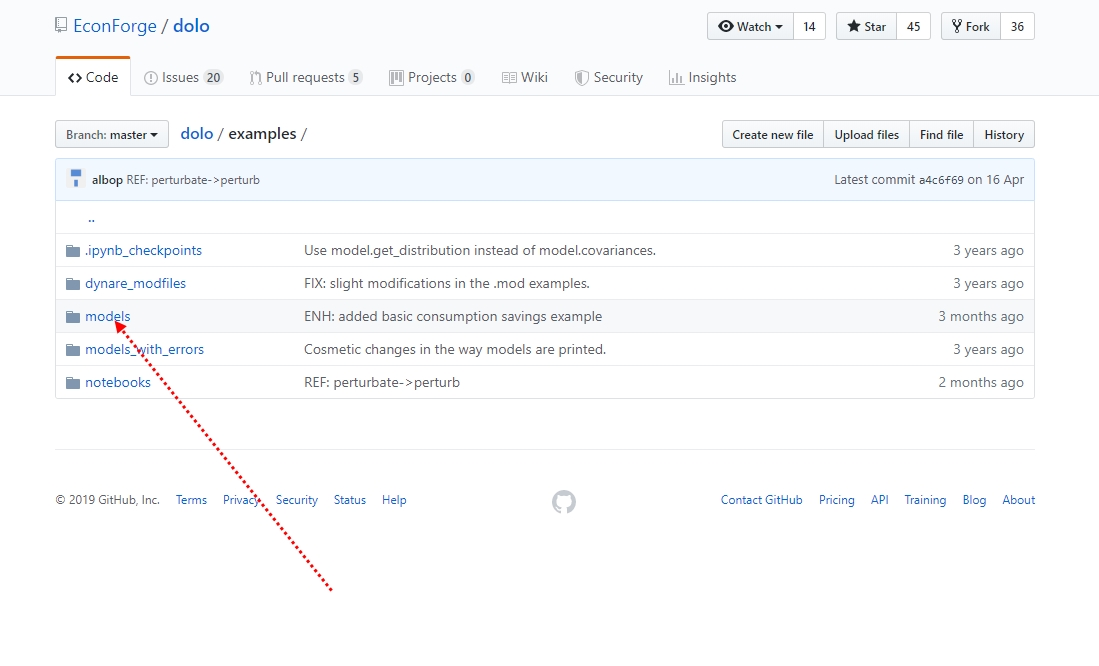
\includegraphics[width=12cm, height= 8cm]{dolo6.jpg}
    \end{frame}
    \begin{frame}{Dolo examples}
        \begin{itemize}
            \item From Pablo's github repository, we can copy and paste a \textit{YAML} example. 
            \item If you make your own \textit{YAML} model file, then you have to be able to run it in your local python. 
            \item To call the model file, you have to get the raw content of files stored in github. This can be done as follows. 
        \end{itemize}
    \end{frame}
     \begin{frame}{}
         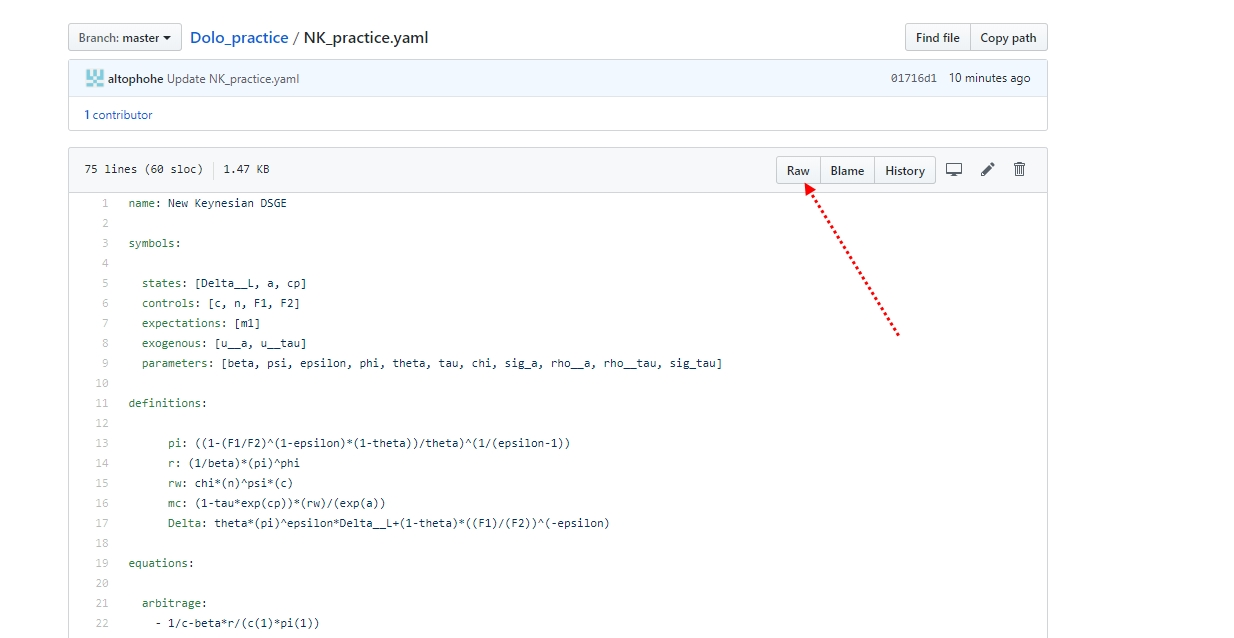
\includegraphics[width=12cm, height= 8cm]{dolo8.jpg}
    \end{frame}
     \begin{frame}{}
         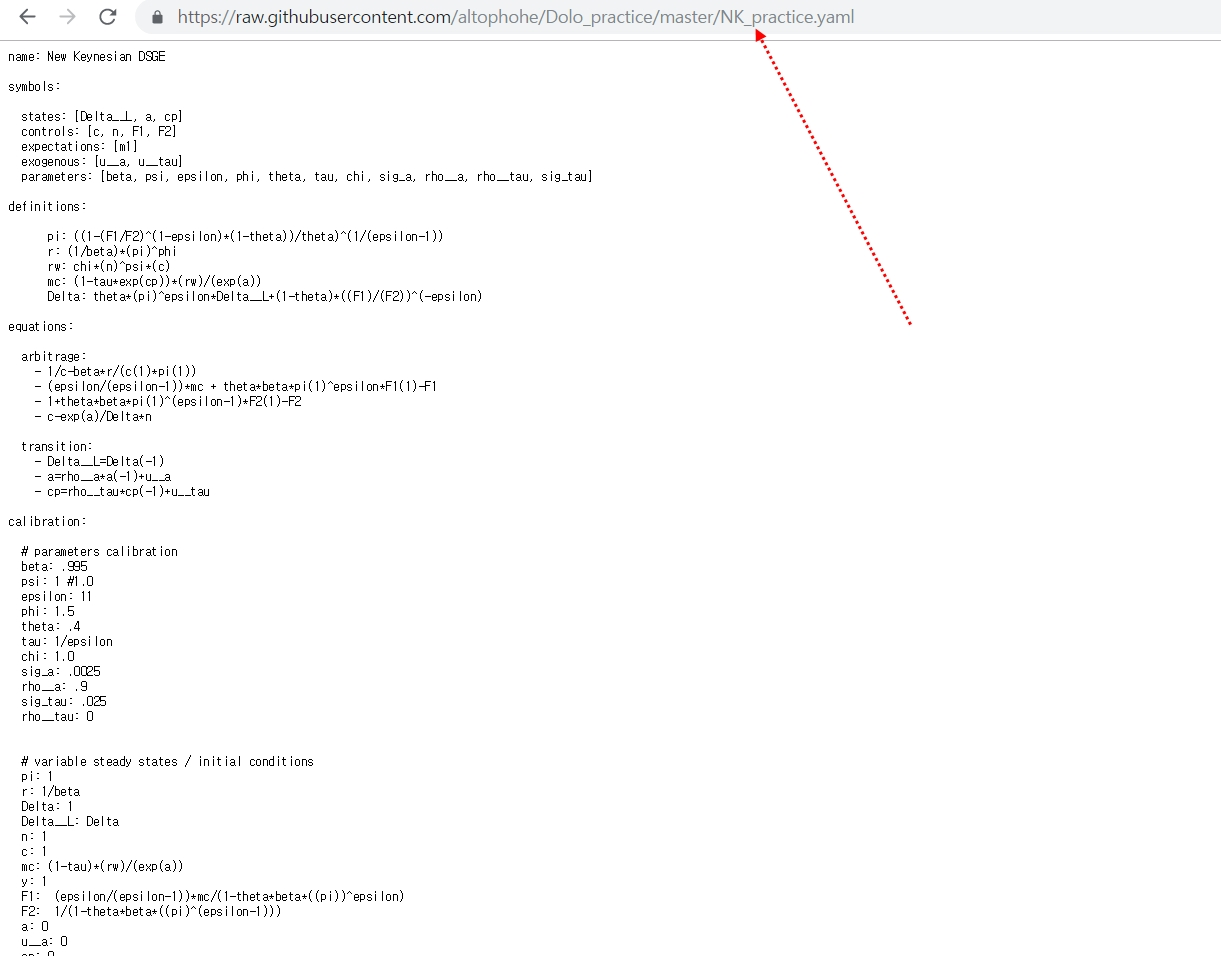
\includegraphics[width=12cm, height= 8cm]{dolo9.jpg}
    \end{frame}
\begin{frame}{Dolo examples}
\begin{itemize}
  
    \item Type on your own \textit{Jupyter notebook} as follows:\\
    
    filename = ('\textit{your yaml raw file address here}')\\
    model = yaml\_ import(filename)\\
    display(model)  

\item If you can see that Jupyter displays the model, it means that the very first step is smoothly done. 
\item The remaining parts are writing your own model properly and run. 
\end{itemize}
\end{frame}
\begin{frame}{Dolo examples}
    \begin{itemize}
        \item Let's choose any example in Pablo's repository and make \textit{YAML} file in your own repository. 
        \item 
    \end{itemize}
\end{frame}
\end{document}
